\section{Entwurf}
\subsection{Geschäftsfälle anhand des BPMN Workflows}
\subsection{Auswahl und Begründung des Datenbankkonzepts}
Die Lernapp \gqq{LearnAhead} benötigt eine Datenbank, um die Lerninhalte des Benutzers zu speichern. Die Datenbank soll die folgenden Anforderungen erfüllen:
\begin{itemize}
    \item Es soll möglich sein, Bilder einfach zu speichern und abzurufen.
    \item Die Datenbank soll gut skalierbar sein, um auch bei vielen Benutzern eine gute Performance zu gewährleisten.
    \item Es müssen gute Frameworks für die Anbindung existieren für die Sprache Kotlin.
    \item Die Datenbank soll in der Cloud gehostet werden, um die Wartungskosten zu minimieren.
    \item Die Datenbank soll möglichst kostenlos sein.
\end{itemize}

\noindent
Hierbei gab es die Entscheidung zwischen einer relationalen und einer NoSQL Datenbank. Da diese für die Speicherung von Bildern zuständig ist, ist eine NoSQL Datenbank die bessere Wahl. In diesem Zusammenhang kam der Anbieter \gqq{Firebase} in Frage. Dieser bietet zwei unterschiedliche Datenbanken an: \gqq{Cloud Firestore} und \gqq{Realtime Database}. Realtime Database wird genutzt, wenn die Datenbank in Echtzeit synchronisiert werden soll. Da dies bei der Lernapp nicht notwendig ist, wurde sich für Cloud Firestore entschieden. Cloud Firestore baut auf den Erfolgen von Realtime Database auf und bietet zusätzlich eine bessere Skalierbarkeit und schnellere Abfragen sind möglich. \cite*{Firestore} Für die Speicherung von Inhalten gibt es den Firebase Storage. Dieser bietet eine einfache Möglichkeit, um Inhalte z.B. Bilder oder Videos zu speichern. \newline

\noindent
Firebase bietet eine gute Anbindung für Kotlin siehe \ref*{Auswahl der Klassenbibliotheken/Frameworks}. Zusätzlich ist Firebase kostenlos, solange die Datenbank nicht zu groß wird. Hierbei kann eine monatliche Anzahl von 50.000 Nutzern, 20.000 Schreibvorgängen und 50.000 Lesevorgängen kostenlos genutzt werden. Der Speicherplatz für den Firebase Storage beträgt 1 GB, welches für die Lernapp ausreichend ist. \cite*{Firebase_Pricing}
\subsection{Auswahl der Klassenbibliotheken/Frameworks} \label{Auswahl der Klassenbibliotheken/Frameworks}
\subsection{Design Patterns für relevante Problemstellungen} \label{Design Patterns für relevante Problemstellungen}
\subsection{Software-Komponenten}
Das System wird zunächst als Gesamtkomposition dargestellt. Anschließend werden die Subsysteme einzeln dargestellt. 
\subsubsection{Gesamtkomposition}
\begin{figure}[H]
    \centering
    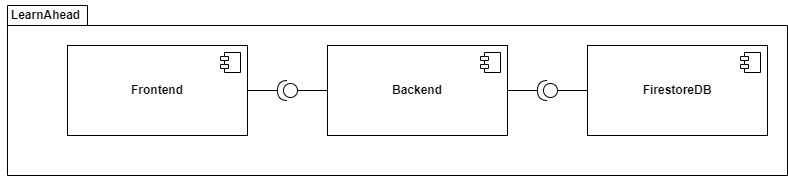
\includegraphics[width=0.8\textwidth]{images/diagramme/Gesamtkomposition.png}
    \caption{Gesamtkomposition}
    \label{fig:Gesamtkomposition}
\end{figure}
\noindent
Die Gesamtkomposition besteht aus den folgenden Subsystemen:
\begin{itemize}
    \item \textbf{Frontend:} Das Frontend ist für die Darstellung der Benutzeroberfläche zuständig. Es kommuniziert mit dem Backend, um Daten abzurufen und zu speichern.
    \item \textbf{Backend:} Das Backend ist für die Verarbeitung und Validierung der Daten zuständig. Es kommuniziert mit der FireStore Datenbank, um Daten abzurufen und zu speichern.
    \item \textbf{FireStoreDB} Die FireStoreDB Komponente ist die Datenbank-Komponente.
\end{itemize}

\noindent
Näheres hierzu im Deployment Diagramm \ref*{Deployment Diagramm} und Klassen Diagramm \ref*{Klassen Diagramm}.
\newpage
\subsubsection{Frontend}
Es gibt zwei Diagramme für das Frontend. Das Diagramm \ref*{fig:FrontendUINavigation} zeigt die Navigation zwischen den einzelnen Pages.
\begin{figure}[H]
    \centering
    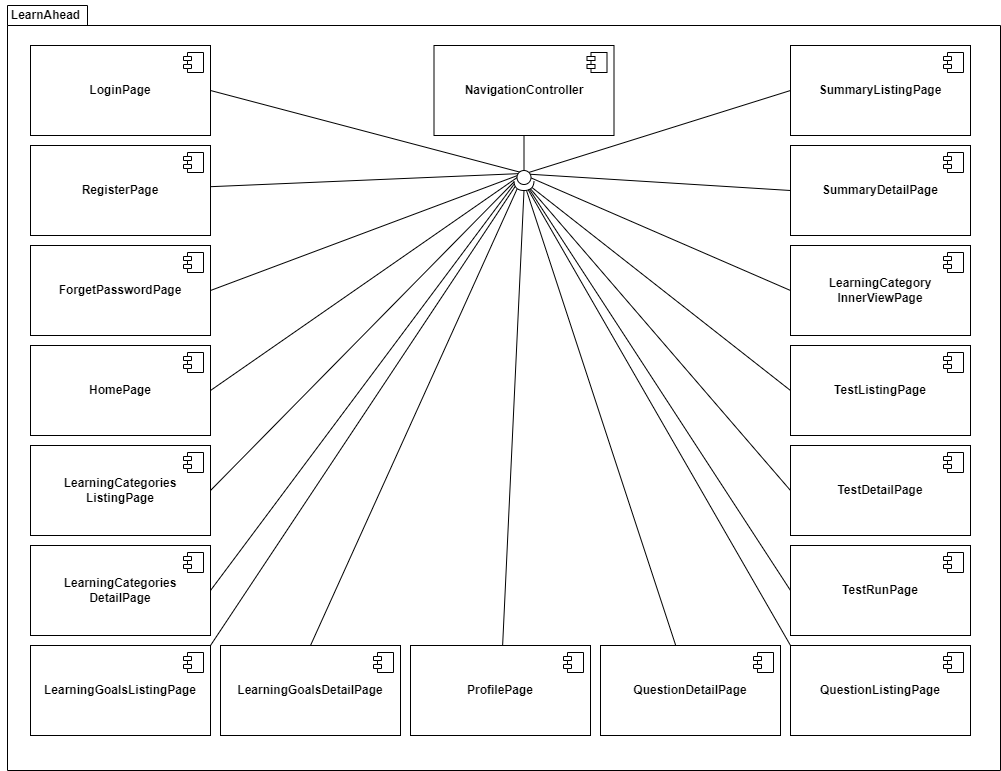
\includegraphics[width=0.8\textwidth]{images/diagramme/FrontEndKomposition.png}
    \caption{Frontend UI Navigation}
    \label{fig:FrontendUINavigation}
\end{figure}
\noindent
Das Diagramm \ref*{fig:FrontendUIViewModel} zeigt die Kommunikation zwischen den einzelnen Pages und dem ViewModel. Hierbei ist zu beachten, dass dieses Diagramm die Kommunikation zwischen den einzelnen Pages und dem ViewModel im allgemeinen zeigt. Das bedeutet, dass jede Page ein zugehöriges ViewModel hat. Die Kommunikation zwischen den einzelnen Pages und dem ViewModel ist prinzipiell immer gleich. Weitere Details sind in Kapitel \ref*{Design Patterns für relevante Problemstellungen} zu finden. \newline
\begin{figure}[H]
    \centering
    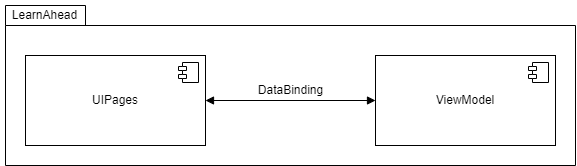
\includegraphics[width=0.8\textwidth]{images/diagramme/UIPagesMitViewModel.png}
    \caption{Frontend UI Kommunikation mit ViewModel}
    \label{fig:FrontendUIViewModel}
\end{figure}
\subsubsection{Backend}
Das Diagramm \ref*{fig:BackendKomposition} zeigt die Komposition des Backends. Hierbei ist zu beachten, dass dieses Diagramm die Komposition des Backends im allgemeinen zeigt. Jedes Objekt, welches in der Datenbank gespeichert wird, hat ein zugehöriges Repository/Model. Die Kommunikation zwischen den verschiedenen Repositories und Modellen verläuft grundsätzlich immer auf die gleiche Weise. Jedes Repository baut auf ein Interface auf, welches die grundlegenden Funktionen für die Kommunikation mit der Datenbank definiert. Die Kommunikation mit der Datenbank folgt über das Repository.
\begin{figure}[H]
    \centering
    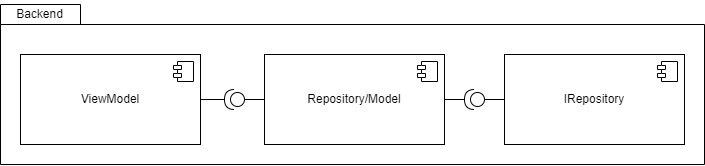
\includegraphics[width=0.8\textwidth]{images/diagramme/Backend.png}
    \caption{Backend Komposition}
    \label{fig:BackendKomposition}
\end{figure}
\subsection{Deployment Diagramm} \label{Deployment Diagramm}
\subsection{Klassen Diagramm} \label{Klassen Diagramm}
\subsection{Aktivitätsdiagramm}
\subsection{Sequenzdiagramme}
\subsection{Prototyp (optional)}